

\tikzset{every picture/.style={line width=0.75pt}} %set default line width to 0.75pt        

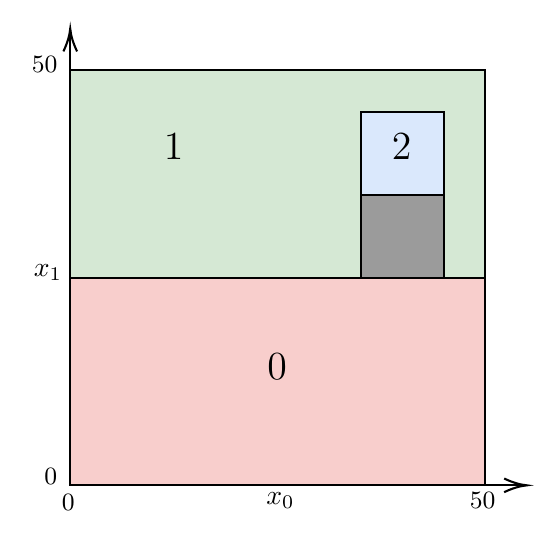
\begin{tikzpicture}[x=0.75pt,y=0.75pt,yscale=-1,xscale=1]
%uncomment if require: \path (0,300); %set diagram left start at 0, and has height of 300

%Shape: Rectangle [id:dp12943827359599314] 
\draw  [fill={rgb, 255:red, 213; green, 232; blue, 212 }  ,fill opacity=1 ] (250,50) -- (450,50) -- (450,150) -- (250,150) -- cycle ;
%Straight Lines [id:da8416607833401318] 
\draw    (250,250) -- (250,32) ;
\draw [shift={(250,30)}, rotate = 90] [color={rgb, 255:red, 0; green, 0; blue, 0 }  ][line width=0.75]    (10.93,-3.29) .. controls (6.95,-1.4) and (3.31,-0.3) .. (0,0) .. controls (3.31,0.3) and (6.95,1.4) .. (10.93,3.29)   ;
%Straight Lines [id:da5577600596159713] 
\draw    (250,250) -- (468,250) ;
\draw [shift={(470,250)}, rotate = 180] [color={rgb, 255:red, 0; green, 0; blue, 0 }  ][line width=0.75]    (10.93,-3.29) .. controls (6.95,-1.4) and (3.31,-0.3) .. (0,0) .. controls (3.31,0.3) and (6.95,1.4) .. (10.93,3.29)   ;
%Straight Lines [id:da17568384394881242] 
\draw    (250,150) -- (450,150) ;
%Shape: Rectangle [id:dp3705541448905584] 
\draw  [fill={rgb, 255:red, 248; green, 206; blue, 204 }  ,fill opacity=1 ] (250,150) -- (450,150) -- (450,250) -- (250,250) -- cycle ;
%Shape: Rectangle [id:dp5334639009219723] 
\draw  [fill={rgb, 255:red, 218; green, 232; blue, 252 }  ,fill opacity=1 ] (390,70) -- (430,70) -- (430,110) -- (390,110) -- cycle ;
%Shape: Rectangle [id:dp05533155300504711] 
\draw  [fill={rgb, 255:red, 155; green, 155; blue, 155 }  ,fill opacity=1 ] (390,110) -- (430,110) -- (430,150) -- (390,150) -- cycle ;

% Text Node
\draw (343.5,185.33) node [anchor=north west][inner sep=0.75pt]  [font=\Large]  {$0$};
% Text Node
\draw (293.6,79) node [anchor=north west][inner sep=0.75pt]  [font=\Large]  {$1$};
% Text Node
\draw (403.5,79.33) node [anchor=north west][inner sep=0.75pt]  [font=\Large]  {$2$};
% Text Node
\draw (343,252) node [anchor=north west][inner sep=0.75pt]    {$x_{0}$};
% Text Node
\draw (231,142) node [anchor=north west][inner sep=0.75pt]    {$x_{1}$};
% Text Node
\draw (244.5,252.67) node [anchor=north west][inner sep=0.75pt]  [font=\small]  {$0$};
% Text Node
\draw (236,240.33) node [anchor=north west][inner sep=0.75pt]  [font=\small]  {$0$};
% Text Node
\draw (230,41.67) node [anchor=north west][inner sep=0.75pt]  [font=\small]  {$50$};
% Text Node
\draw (441,252) node [anchor=north west][inner sep=0.75pt]  [font=\small]  {$50$};


\end{tikzpicture}
